%!TEX program = xelatex
\documentclass[12pt]{article}

% ---------- IDIOMA Y FUENTE ----------
\usepackage{fontspec} 
\usepackage[spanish, es-tabla]{babel} 
% --- Cambiar "Cuadro" por "Tabla" ---
\addto\captionsspanish{\renewcommand{\tablename}{Tabla}}
\setmainfont{TeX Gyre Termes}

% ---------- PAQUETES MATEMÁTICOS Y FÍSICOS ----------
\usepackage{amsmath,amssymb,amsfonts}
\usepackage{physics}

% ---------- GRÁFICOS Y COLORES ----------
\usepackage{xcolor}
\usepackage{graphicx}
\usepackage{tikz}
\usetikzlibrary{babel} 
\usepackage{tikz-3dplot}
\usetikzlibrary{shapes, arrows, positioning}
\usetikzlibrary{arrows.meta, angles, quotes, calc, patterns} 
\usetikzlibrary{shapes.geometric} 
\usetikzlibrary{decorations.markings}

% ---------- CÓDIGO (LISTINGS) ----------
\usepackage{listings}
\definecolor{codegreen}{rgb}{0,0.6,0}
\definecolor{codegray}{rgb}{0.95,0.95,0.95}
\definecolor{codepurple}{rgb}{0.58,0,0.82}
\definecolor{backcolour}{rgb}{0.96,0.96,0.96}

\lstdefinestyle{pythonstyle}{
    backgroundcolor=\color{backcolour},   
    commentstyle=\color{codegreen},
    keywordstyle=\color{magenta},
    numberstyle=\tiny\color{gray},
    stringstyle=\color{codepurple},
    basicstyle=\ttfamily\small,          
    breakatwhitespace=false,         
    breaklines=true,                     
    captionpos=b,                    
    keepspaces=true,                 
    numbers=left,                        
    numbersep=5pt,                  
    showspaces=false,                
    showstringspaces=false,
    showtabs=false,                  
    tabsize=4,
    language=Python                      
}
\lstset{style=pythonstyle}

% ---------- DISEÑO Y ESTILO ----------
\usepackage{geometry}
\geometry{letterpaper, margin=2cm, headheight=15pt}
\usepackage{fancyhdr} 
\usepackage{lastpage}
\usepackage{wrapfig}
\usepackage{multicol}
\usepackage{enumitem}
\usepackage{framed}
\usepackage{etoolbox}

% ---------- TCOLORBOX ----------
\usepackage[most,skins,theorems]{tcolorbox}

% --- Caja para Definiciones Formales ---
\newtcolorbox{definicion}[1][]{
  enhanced,
  breakable, 
  colback=blue!5!white,
  colframe=blue!75!black,
  fonttitle=\bfseries,
  title={Definición: #1},
  arc=2mm,
  boxrule=0.8pt,
  drop shadow=black!10!white
}

% --- Caja para Tareas ---
\newtcolorbox{problemas}[1][]{
  enhanced,
  breakable, 
  colback=violet!6!white,       
  colframe=violet!45!white,     
  coltitle=violet!40!black,     
  fonttitle=\bfseries,
  title={Problemas: #1},
  arc=2.5mm,                    
  boxrule=0.8pt,
  drop shadow=black!8!white     
}

% --- Caja Libre Verde Menta ---
\newtcolorbox{cajaflex}[1][]{
  enhanced,
  breakable, 
  colback=teal!5!white,       
  colframe=teal!50!black,     
  coltitle=teal!10!white,     
  fonttitle=\bfseries,
  code={\ifblank{#1}{}{\tcbset{title={#1}}}},
  arc=2.5mm,                  
  boxrule=0.8pt,
  drop shadow=black!8!white   
}

% ---------- TABLAS Y ELEMENTOS EXTRA ----------
\usepackage{booktabs}   
\usepackage{pifont}     
\usepackage{array}      
\usepackage{caption}    
\newcommand{\lapiz}{\ding{46}\ }

% ---------- CONFIGURACIÓN DE ENCABEZADOS (ITM) ----------
\newcommand{\logo}{
\includegraphics[height=3cm]{escudoitm}}
\newcommand{\escola}{Facultad de Ciencias Exactas y Aplicadas}
\newcommand{\disc}{Física Computacional 1}
\newcommand{\auth}{Robinson Longas Bedoya}
\newcommand{\emaill}{\url{robinsonlongas@itm.edu.co}}
\newcommand{\email}{\url{robinsonlongas3586@correo.itm.edu.co}}
\newcommand{\cabec}{Física Computacional 1}

% ---------- ENLACES Y PDF ----------
\usepackage{hyperref}

\definecolor{myblue}{RGB}{20, 20, 120}
\definecolor{myred}{RGB}{220, 30, 30}
\definecolor{mygreen}{RGB}{0, 130, 60}

% Personalización de nombres para \autoref
\def\tableautorefname{Tabla}
\def\figureautorefname{Figura}
\def\equationautorefname{Ecuación}
\def\sectionautorefname{Sección}

\hypersetup{
    colorlinks=true,
    linkcolor=blue,
    urlcolor=blue,
    citecolor=blue,
    pdftitle={Física Computacional 1 -- Robinson Longas Bedoya},
    pdfauthor={Robinson Longas Bedoya}
}

% Configuración de estilos de página
\pagestyle{fancy}
\fancyhf{} 

\fancypagestyle{firstpage}{
    \fancyhead[L]{\logo}
    \fancyhead[R]{
        \textsf{\escola \\} 
        \textsf{\disc \\}
        \textsf{\auth \\}
        \textsf{\email \\} 
        \textsf{\emaill}     
    }
    \fancyfoot[R]{\scriptsize Página \thepage~de \pageref{LastPage}}
    \renewcommand{\headrulewidth}{0pt} 
    \renewcommand{\footrulewidth}{0.4pt} 
}

\fancyhead[L]{\textsf{\scriptsize \cabec\ -- \auth\ -- \email\ -- \emaill}}
\fancyfoot[R]{\scriptsize Página \thepage~de \pageref{LastPage}}
\renewcommand{\headrulewidth}{0.4pt} 
\renewcommand{\footrulewidth}{0.4pt} 

\setlength{\parskip}{0.3em}

\begin{document}
		\thispagestyle{firstpage}
		\vspace*{1.5cm}
	
	\begin{center}
		\rule{\textwidth}{0.4pt}
	\end{center}
	
	\begin{itemize}[leftmargin=*,label=\textcolor{red}{\ensuremath{\blacktriangleright}}]
		\item \textbf{Solución de ecuaciones no lineales y trascendentes}
		\item \textbf{Raíces de polinomios}
	\end{itemize}
	
	\noindent
	\textbf{\underline{Bibliografía}}
	\begin{itemize}[leftmargin=*, label={\textcolor{blue}{$\bullet$}}]
		\item \textit{Computational Physics}, Mark Newman.
        \item \textit{Programming for computations - Python}, Evein Linge and Petter Langtangen. 
        \item \textit{Computational Physics with Python}, Eric Ayars. 
        \item \textit{Computational mathematics: An introduction to 
        Numerical Analysis and Scientific Computing  with Python}, Dimitrios Mitsotakis. 
        \item \textit{Computational physics: problem solving with Python}, 
        Rubin H. Landau, Manuel J. Páez and Cristian C. Bordeianu.
    \end{itemize}
     
    

\section*{\textcolor{red}{\textit{Solución de ecuaciones no lineales y trascendentes}}}

Suponga que se lanza un cuerpo con una velocidad inicial inicial 
$\vec v_0$ formando un ángulo $\theta$ con la horizontal.
En Física básica se muestra que las ecuaciones de movimiento para este
sistema son
\begin{align*}
    x(t) &= x_0 + v_0\cos\theta t\,, \\
    y(t) &= y_0 + v_0\sin\theta t  - \frac{g}{2} t^2 \,.
\end{align*}

Si queremos saber el tiempo en que el cuerpo cae al piso de nuevo,
debemos resolver la ecuación $y(T) = 0$. Cuya solución 
puede escribirse como
\begin{align*}
    T = \frac{v_0 \sin\theta + \sqrt{(v_0 \sin\theta)^2 + 2 g y_0}}{g}\,.
\end{align*}
Con ese tiempo, podemos escribir el alcance horizontal del proyectil 
como
\begin{align}
    \label{eq:alcance_maximo}
    x(\theta) = x_0 + \frac{v_0 \cos\theta}{g} 
    \left[ v_0 \sin\theta + \sqrt{(v_0 \sin\theta)^2 + 2 g y_0} \right]
\end{align}
La ecuación \eqref{eq:alcance_maximo} es una ecuación no 
lineal en $\theta$. Si de entrada conocemos el ángulo de 
lanzamiento, simplemente lo reemplazamos en dicha ecuación.
Pero, en la mayoría de casos, podemos medir el alcance horizontal
y queremos determinar el ángulo de lanzamiento. Es decir, 
dado $x$, queremos saber $\theta$. Su solución requiere de 
métodos numéricos.

La forma más simple de hacerlo es graficar el lado izquierdo y 
el lado derecho para mirar en donde se cruzan. Por otro lado, 
existen métodos para hacerlo: \textit{bisección, Newton, secante}. 
En nuestro curso no vamos a estudiar con detalle estos métodos,
vamos a utilizar las librerías científicas de Python.
%===========Figura montaje experimental ====================
%
\begin{figure}[htbp]
\centering
\begin{tikzpicture}[scale=1.1, >=latex]
    
    % Pata y superficie de la mesa
    \draw[thick, fill=gray!10] (0,0) -- (0,1.8) -- (-1.2,1.8) -- (-1.2,2.1) -- (2.0,2.1) -- (2.0,1.8) -- (0.8,1.8) -- (0.8,0) -- cycle;
    
    % Soporte vertical del lanzador
    \draw[thick, fill=gray!30] (1.5,2.1) rectangle (1.9,4.2);
    \draw[thick, fill=white] (1.65,2.4) rectangle (1.75,3.9); % Ranura central del soporte
    
    % Prensa en C (Clamp)
    \draw[thick, fill=gray!50] (1.3,1.6) -- (2.2,1.6) -- (2.2,2.3) -- (1.9,2.3) -- (1.9,1.8) -- (1.3,1.8) -- cycle;
    \draw[thick] (1.7,1.6) -- (1.7,0.9);
    \draw[thick, fill=black] (1.5,0.9) rectangle (1.9,1.0);
    \draw[thick] (1.7,0.7) circle (0.15); % Manivela
    
    % Cañón/Lanzador inclinado (Ángulo de ~30 grados)
    \begin{scope}[shift={(1.7,3.9)}, rotate=30]
        \draw[thick, fill=gray!80] (-0.3,-0.3) rectangle (1.2,0.3);
        \draw[thick, fill=black!20] (0.2,0) circle (0.15); % Esfera/Proyectil dentro
        \draw[thick] (-0.2,-0.3) -- (-0.2,-0.6) node[circle, fill=black, inner sep=1pt]{}; % Plomada
    \end{scope}

    % --- PUNTOS CLAVE Y COORDENADAS ---
    % Origen de lanzamiento (x0, y0)
    \coordinate (P0) at (2.0, 4.2); % Punto de salida
    \coordinate (Suelo) at (2.0, 0);

    % --- ELEMENTOS DEL LANZAMIENTO PARABÓLICO ---
    
    % 1. Línea horizontal de referencia para el ángulo theta
    \draw[dashed, black!70] (P0) -- ($(P0) + (2.5,0)$);
    
    % 2. Vector de velocidad inicial v0
    \draw[->, thick] (P0) -- ($(P0) + (30:2.8)$) node[above left] {$v_0$};
    
    % 3. Arco y etiqueta del ángulo theta
    \path (P0) ++(2.0,0) coordinate (RefH);
    \path (P0) ++(30:2.0) coordinate (RefV);
    \draw pic[draw, "$\theta$", angle radius=1.2cm, angle eccentricity=1.2] {angle = RefH--P0--RefV};

    % 4. Trayectoria Parabólica (punteada)
    % Curva Bezier que simula la parábola desde x0 hasta tocar el suelo en x_final
    \draw[dashed, domain=0:6.5, samples=100, variable=\x] 
    plot ({\x + 2.0}, {-0.09*\x*\x + tan(30)*\x + 4.2});
    
    % Punto de impacto en el suelo
    \coordinate (Impacto) at (8.5, 0);

    % --- COTAS Y DIMENSIONES (x, y0, x0) ---
    
    % Línea de suelo de referencia
    \draw[dashed, black!60] (-0.5,0) -- (Impacto);

    % Cota de altura inicial y0
    \draw[<->] (3.0, 0) -- (3.0, 4.2) node[midway, fill=white] {$y_0$};
    
    % Cota de alcance horizontal x (desde el eje vertical de salida hasta el impacto)
    \draw[<->] (Suelo) -- (Impacto) node[midway, above] {$x$};
    
    % opcional: marcar x0 desde el origen absoluto si se desea
    %\draw[<->] (0, -0.3) -- (2.0, -0.3) node[midway, below] {$x_0$};

\end{tikzpicture}
\caption{Montaje de laboratorio para lanzamiento de proyectiles con altura inicial $y_0$.}
\end{figure}
%
%
\begin{lstlisting}[language=Python, captionpos=t, title=\texttt{raices\_parabolico.py}]
""" En este programa se utiliza la librería scipy 
    para encontrar los ángulos de lanzamiento de un cuerpo para 
    una altura máxima y una distancia horizontal máxima"""

import scipy as sp
import numpy as np
import matplotlib.pyplot as plt

def x_max(theta, x0=0., y0 = 0., v0 = 3.5, g = 9.8):
    """ función para encontrar el desplazamiento máximo horizontal. 
    Variables de entrada. theta:  ángulo en metros. y0: altura inicial en metros.
    v0: magnitud de la velocidad inicial en m/s. g: aceleración gravedad en m/s^2"""
    sintheta = np.sin(np.radians(theta))
    costheta = np.cos(np.radians(theta))
    prefactor = ( v0 * costheta )/g
    return x0 + prefactor * (v0 * sintheta + np.sqrt(v0**2 * sintheta**2 + 2*g*y0) )

def y_max(theta, y0 = 0., v0 = 3.5, g = 9.8):
    """ función para encontrar la altura máxima. 
    Variables de entrada. theta:  ángulo en metros. y0: altura inicial en metros.
    v0: magnitud de la velocidad inicial en m/s. g: aceleración gravedad en m/s^2"""
    sintheta = np.sin(np.radians(theta))
    return y0 + 1/(2.*g) * v0**2 * sintheta**2

def f_x(theta, xmaximo, x0, y0, v0, g):
    """Función asociada al alcance horizontal máximo:  xmaximo - x_max(theta,...) = 0"""
    return x_max(theta, x0, y0, v0, g) - xmaximo

def f_y(theta, ymaxima, y0, v0, g):
    """Función asociada a la altura máxima:  ymaximo - y_max(theta,...) = 0"""
    return y_max(theta, y0, v0, g) - ymaxima


if __name__ == "__main__":
    y0 = 1.5      # Altura inicial (m)
    x0 = 0.0      # Posición inicial (m)
    v0 = 35.0     # Velocidad inicial (m/s)
    g = 9.8       # Gravedad (m/s^2)
    xmaximo = 89.0 # Alcance máximo (m)

    angulos = np.linspace(0, 90, 300)
    alcancesx = x_max(angulos, x0, y0, v0, g)

    plt.figure(figsize=(8, 5))
    plt.plot(angulos, alcancesx, label=r'$x_{\mathrm{max}}(\theta)$', color='blue', lw=2)
    plt.axhline(xmaximo, color='red', linestyle='--', label=rf'$x_{{max}} = $ {xmaximo} m')
    plt.title(f'Alcance Horizontal vs Ángulo ($v_0 = {v0}$ m/s, $y_0 = {y0}$ m)')
    plt.xlabel(r'$\theta$ (grados)')
    plt.ylabel('$x$ (m)')
    plt.grid(True, linestyle=':', alpha=0.7)
    plt.legend()
    plt.tight_layout()

    try: 
        sol1 = sp.optimize.root_scalar(f_x, args=(xmaximo, x0, y0, v0, g), bracket=[0, 45], method='brentq')
        sol2 = sp.optimize.root_scalar(f_x, args=(xmaximo, x0, y0, v0, g), bracket=[45, 90], method='brentq') 

        res1 = f_x(sol1.root, xmaximo, x0, y0, v0, g)
        res2 = f_x(sol2.root, xmaximo, x0, y0, v0, g)

        print(f"\n--- Ángulos con que se debe lanzar la pelota para un alcance máximo de = {xmaximo} metros---")
        print(f"Ángulo 1  : {sol1.root:.4f}°| Error: {abs(res1):.2e} m  | Iteraciones: {sol1.iterations}")
        print(f"Ángulo 2 : {sol2.root:.4f}° | Error: {abs(res2):.2e} m | Iteraciones: {sol2.iterations}")

    except ValueError:
        # Ocurre un error si no encuentra soluciones 
        alcance_max_posible = np.max(alcancesx)
        print(f"\n[Error] El alcance deseado de {xmaximo} m es físicamente inalcanzable.")
        print(f"El alcance máximo posible con v0={v0} m/s y y0={y0} m es de {alcance_max_posible:.2f} m.")    
    
    #plt.savefig('../Clases/Herramientas_Python/alcance_vs_angulo.pdf', bbox_inches='tight')
    plt.show() 
\end{lstlisting}
%
\begin{figure}[htbp]
    \centering
    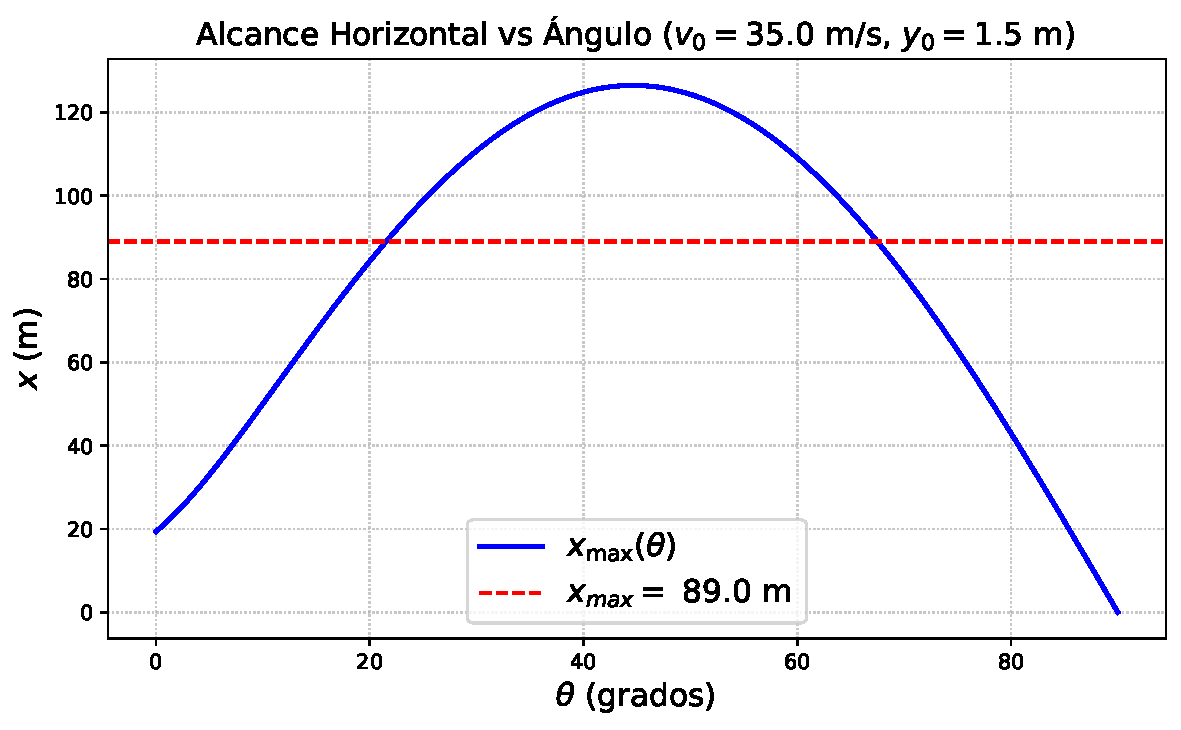
\includegraphics[width=0.8\textwidth]{alcance_vs_angulo.pdf}
    \caption{Alcance máximo en función del ángulo de lanzamiento.}
\end{figure}

\subsection*{\textcolor{blue}{\textit{Ejemplo:}}} Encontremos 
la solución de la ecuación $x = - \ln(x) \implies 
f(x) = x + \ln(x) = 0$ de manera numérica.
\begin{cajaflex}[La función $W$ de Lambert]
    En matemáticas se define la función de Lambert $W$ como 
    $$  z = W(z)e^{W(z)} $$
    Noten pues que en nuestro caso, con 
    $$x+\ln x= 0\implies x = -\ln x \implies e^x = e^{-\ln x} = e^{\ln (x)^{-1}}
    = \frac{1}{x}\implies xe^x =1$$
    Si comparamos con función $W$ podemos ver que la solución a la ecuación 
    $ue^u = y$ es $u = W(y)$. Luego, la solución a la ecuación $xe^x = 1$ es $W(1)$
\end{cajaflex}
\begin{lstlisting}[language=Python, captionpos=t, title=\texttt{raices\_xlnx.py}]
import scipy as sp
import numpy as np
import matplotlib.pyplot as plt

def f(x):
    return x + np.log(x)

def df(x):
    return 1 + 1/x

x = np.linspace(0.01, 10, 100)
fx = f(x)

plt.figure(figsize=(8, 5))
plt.plot(x, x, color='blue', lw=2, label=rf'$f(x) = x$' )
plt.plot(x, -np.log(x), color='red', linestyle='--', label=rf'$f(x)= - \ln({{x}})  $',lw=2)
plt.ylabel(r'$f(x)$',fontsize=15)
plt.xlabel(r'$x$ ',fontsize=15)
plt.grid(True, linestyle=':', alpha=0.7)
plt.legend(fontsize=15)
plt.tight_layout()

sol_brent = sp.optimize.root_scalar(f, bracket=[0.1, 1.0], method='brentq')
sol_secante = sp.optimize.root_scalar(f, x0=1.0, method='secant')
sol_bisect  = sp.optimize.root_scalar(f, bracket=[0.1, 1.0], method='bisect',xtol=1e-8)
sol_newton  = sp.optimize.root_scalar(f, x0=1.0, fprime=df, method='newton')
sol_lambert = np.real(sp.special.lambertw(1))

metodos = [
    ("Brent (brentq)", sol_brent.root, sol_brent.iterations, sol_brent.function_calls),
    ("Bisección", sol_bisect.root, sol_bisect.iterations, sol_bisect.function_calls),
    ("Secante", sol_secante.root, sol_secante.iterations, sol_secante.function_calls),
    ("Newton", sol_newton.root, sol_newton.iterations, sol_newton.function_calls),
    ("Lambert W", sol_lambert, 1, 1)
]

print(f"{'Método':<18} | {'Raíz Hallada':<14} | {'Residuo f(x)':<14} | {'Iteraciones':<12} | {'Llamadas f(x)':<14}")
print("-" * 80)
for nombre, raiz, iters, nfev in metodos:
    residuo = abs(f(raiz))
    print(f"{nombre:<18} | {raiz:<14.8f} | {residuo:<14.2e} | {iters:<12} | {nfev:<14}")

plt.savefig('../Clases/Herramientas_Python/xlnx.pdf', bbox_inches='tight')
plt.show()
\end{lstlisting}
%  
%
\begin{figure}[htbp]
    \centering
    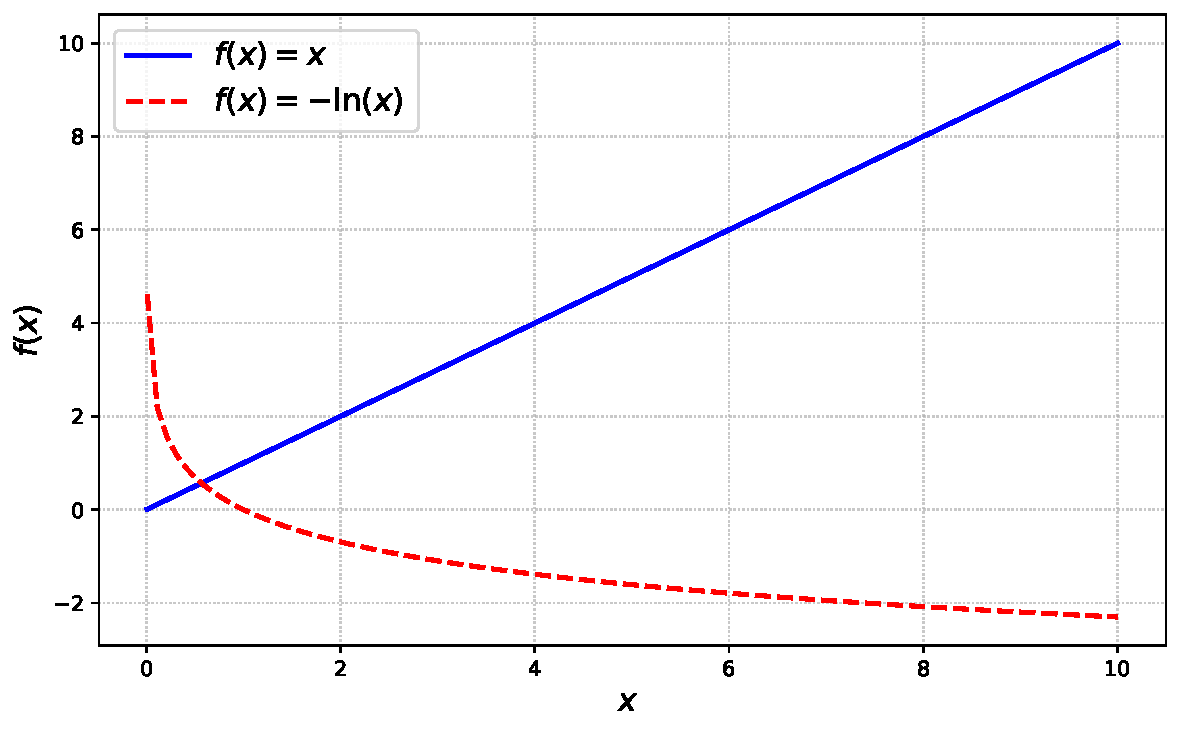
\includegraphics[width=0.8\textwidth]{xlnx.pdf}
    \caption{Gráfica de $x$ y $-\ln(x)$ vs $x$.}
\end{figure}
%
\begin{cajaflex}[\texttt{Resumen de argumentos de root\_scalar por método}]

$\blacklozenge$ Acceda a la documentación oficial \lstinline|scipy.optimize.root_scalar| 
\href{https://docs.scipy.org/doc/scipy/reference/generated/scipy.optimize.root_scalar.html}{dando clic aquí}.

\lstinline|sol=sp.optimize.root_scalar(f, args=(), method=None, bracket=None, fprime=None,| \\
\lstinline|                           fprime2=None, x0=None, x1=None, xtol=None, rtol=None,|\\ 
\lstinline|                           maxiter=None, options=None)|\\

\textcolor{teal!60!black}{\rule{\linewidth}{0.8pt}}

\vspace{0.1cm}

\lstinline|root_scalar(f, bracket=[a,b], method='brentq')| \quad \hfill \text{\small (Método de Brent)} \\
\lstinline|root_scalar(f, bracket=[a,b], method='bisect')| \quad \hfill \text{\small (Método de Bisección)} \\
\lstinline|root_scalar(f, x0=x0, x1=x1, method='secant')| \quad \hfill \text{\small (Método de la Secante)} \\
\lstinline|root_scalar(f, x0=x0, fprime=df, method='newton')| \quad \hfill \text{\small (Método de Newton-Raphson)}

\textcolor{teal!60!black}{\rule{\linewidth}{0.8pt}}

\vspace{0.1cm}

\subsubsection*{\textcolor{teal!70!black}{1. Parámetros Generales}}
\begin{itemize}
    \item \textbf{\texttt{f}:} La función escalar $f(x)$ cuya raíz se desea encontrar.
    \item \textbf{\texttt{args}:} Tupla con argumentos adicionales para $f(x, a, b)$ si la función los requiere (\texttt{args=(a, b)}).
    \item \textbf{\texttt{xtol} / \texttt{rtol}:} Tolerancia absoluta y relativa esperada para el error en $x$.
    \item \textbf{\texttt{maxiter}:} Número máximo de iteraciones permitidas antes de detener el algoritmo.
    \item \textbf{\texttt{options}:} Diccionario de opciones adicionales específicas del método (p. ej., \texttt{\{'disp': True\}}).
\end{itemize}

\subsubsection*{\textcolor{teal!70!black}{2. Métodos}}

\begin{itemize}
    \item \textbf{Método de Brent (\texttt{method='brentq'}):}
    Algoritmo híbrido que combina bisección, secante e interpolación 
    cuadrática inversa. Es el método estándar de propósito general
    para funciones continuas en un intervalo.
    Requiere obligatoriamente 
    un cambio de signo en el intervalo ($f(a) \cdot f(b) < 0$). 
    Ofrece convergencia superlineal con la garantía de estabilidad de 
    la bisección.
   
    \begin{itemize}  
        \item \textbf{\texttt{bracket}:} Intervalo $[a, b]$ obligatorio donde $f(a) \cdot f(b) < 0$.
        \item \textit{Parámetros opcionales:} \texttt{args}, \texttt{xtol}, \texttt{rtol}, \texttt{maxiter}.
    \end{itemize}

    \item \textbf{Método de Bisección (\texttt{method='bisect'}):}
    Divide reiteradamente el intervalo a la mitad y selecciona el 
    subintervalo donde ocurre el cambio de signo.
    
    \begin{itemize}
        \item \textbf{\texttt{bracket}:} Intervalo $[a, b]$ obligatorio con cambio de signo ($f(a) \cdot f(b) < 0$).
        \item \textit{Parámetros opcionales:} \texttt{args}, \texttt{xtol}, \texttt{rtol}, \texttt{maxiter}.
    \end{itemize}

    \item \textbf{Método de la Secante (\texttt{method='secant'}):}
    Método abierto que aproxima la derivada $f'(x)$ mediante la 
    pendiente de la recta secante formada por dos puntos.
    No requiere intervalo cerrado con cambio de signo ni derivada 
    analítica. Se recomienda pasar dos semillas 
    iniciales (\texttt{x0} y \texttt{x1}); si se omite \texttt{x1}, 
    SciPy genera automáticamente un punto cercano $x_1 = x_0 + \delta$.
    \begin{itemize}
        \item \textbf{\texttt{x0}:} Primer punto o semilla inicial (obligatorio).
        \item \textbf{\texttt{x1}:} Segundo punto inicial (recomendado para definir el paso de la secante).
        \item \textit{Parámetros opcionales:} \texttt{args}, \texttt{xtol}, \texttt{rtol}, \texttt{maxiter}.
    \end{itemize}

    \item \textbf{Método de Newton-Raphson (\texttt{method='newton'}):}
    Implementa la iteración $x_{k+1} = x_k - f(x_k)/f'(x_k)$ utilizando la 
    tangente a la curva en el punto actual.
    Presenta convergencia cuadrática cerca de la raíz. 
    Requiere pasar explícitamente la función derivada $f'(x)$ mediante 
    el parámetro \texttt{fprime}.
    \begin{itemize}
        \item \textbf{\texttt{x0}:} Punto o semilla inicial (obligatorio).
        \item \textbf{\texttt{fprime}:} Función de Python que retorna la primera derivada $f'(x)$ (obligatorio).
        \item \textit{Parámetros opcionales:} \texttt{fprime2} (para Halley), \texttt{args}, \texttt{xtol}, \texttt{rtol}, \texttt{maxiter}.
    \end{itemize}
\end{itemize}

\subsubsection*{\textcolor{teal!70!black}{3. Atributos del objeto de 
retorno (\texttt{sol})}}
\begin{itemize}
    \item \textbf{\texttt{sol.root}:} Valor numérico de la raíz encontrada.
    \item \textbf{\texttt{sol.converged}:} Booleano que indica si el algoritmo convergió con éxito (\texttt{True}/\texttt{False}).
    \item \textbf{\texttt{sol.iterations}:} Número de iteraciones ejecutadas.
    \item \textbf{\texttt{sol.function\_calls}:} Número total de evaluaciones realizadas a la función $f(x)$.
\end{itemize}

\end{cajaflex}

\section*{\textcolor{red}{\textit{Raíces de polinomios}}}

El problema de encontrar las $n$ raíces de un polinomio de grado $n$ es una tarea 
computacionalmente relevante. Los métodos analíticos que nos enseñan tradicionalmente 
se vuelven imprácticos para $n > 3$.

Por ejemplo, encontrar las raíces de $p(x) = x^2 - 2x + 1$ es trivial, pero determinar 
las raíces de 
%
\begin{align*}
   p(x) = 3x^7 - 4x^5 + 6x^2 - x + 3
\end{align*}
%
requiere de métodos numéricos. En Python disponemos de dos aproximaciones con NumPy: 
la función clásica \lstinline|np.roots| y la moderna \lstinline|np.polynomial.Polynomial|.
Puede encontrar la documentación 
\href{https://numpy.org/doc/stable/reference/routines.polynomials.html}{dando clic aquí}.
%
\begin{lstlisting}[language=Python, captionpos=t, title=\texttt{raices\_polinomios.py}]
import numpy as np
import matplotlib.pyplot as plt

#======= Polinomio: 3x^7 - 4x^5 + 0x^4 + 0x^3 + 6x^2 - x + 3 = 0 ==============

coeff = [3, -1, 6, 0, 0, -4, 0, 3] # note el orden, de menor a mayor
p = np.polynomial.Polynomial(coeff)
raices_p = p.roots()
print("Polinomio:")
print(p)
print("\nRaíces encontradas:")
for i, r in enumerate(raices_p):
    valorevaluado = p(r)
    print(f"  x_{i+1} = {r:.4f}")
    print(f"|residuo|: {abs(valorevaluado):.2e}")

# ===== plot ========
x = np.linspace(-2, 2, 400)
y = np.polyval(coeff, x)
plt.figure(figsize=(10, 7))
plt.plot(x, y, color='red', linestyle='-', label=rf'$p(x)= 3x^7 - 4x^5 + 6x^2 - x + 3 $',lw=2)
plt.xlabel(r'$x$ ',fontsize=20)
plt.grid(True, linestyle=':', alpha=0.7)
plt.legend(fontsize=20)
plt.tick_params(axis='both', which='both', labelsize=17) # tamño de los ejes
plt.tight_layout()   
plt.savefig('../Clases/Herramientas_Python/polinomio.pdf', bbox_inches='tight')

plt.show()
\end{lstlisting}
%

%
\begin{figure}[htbp]
    \centering
    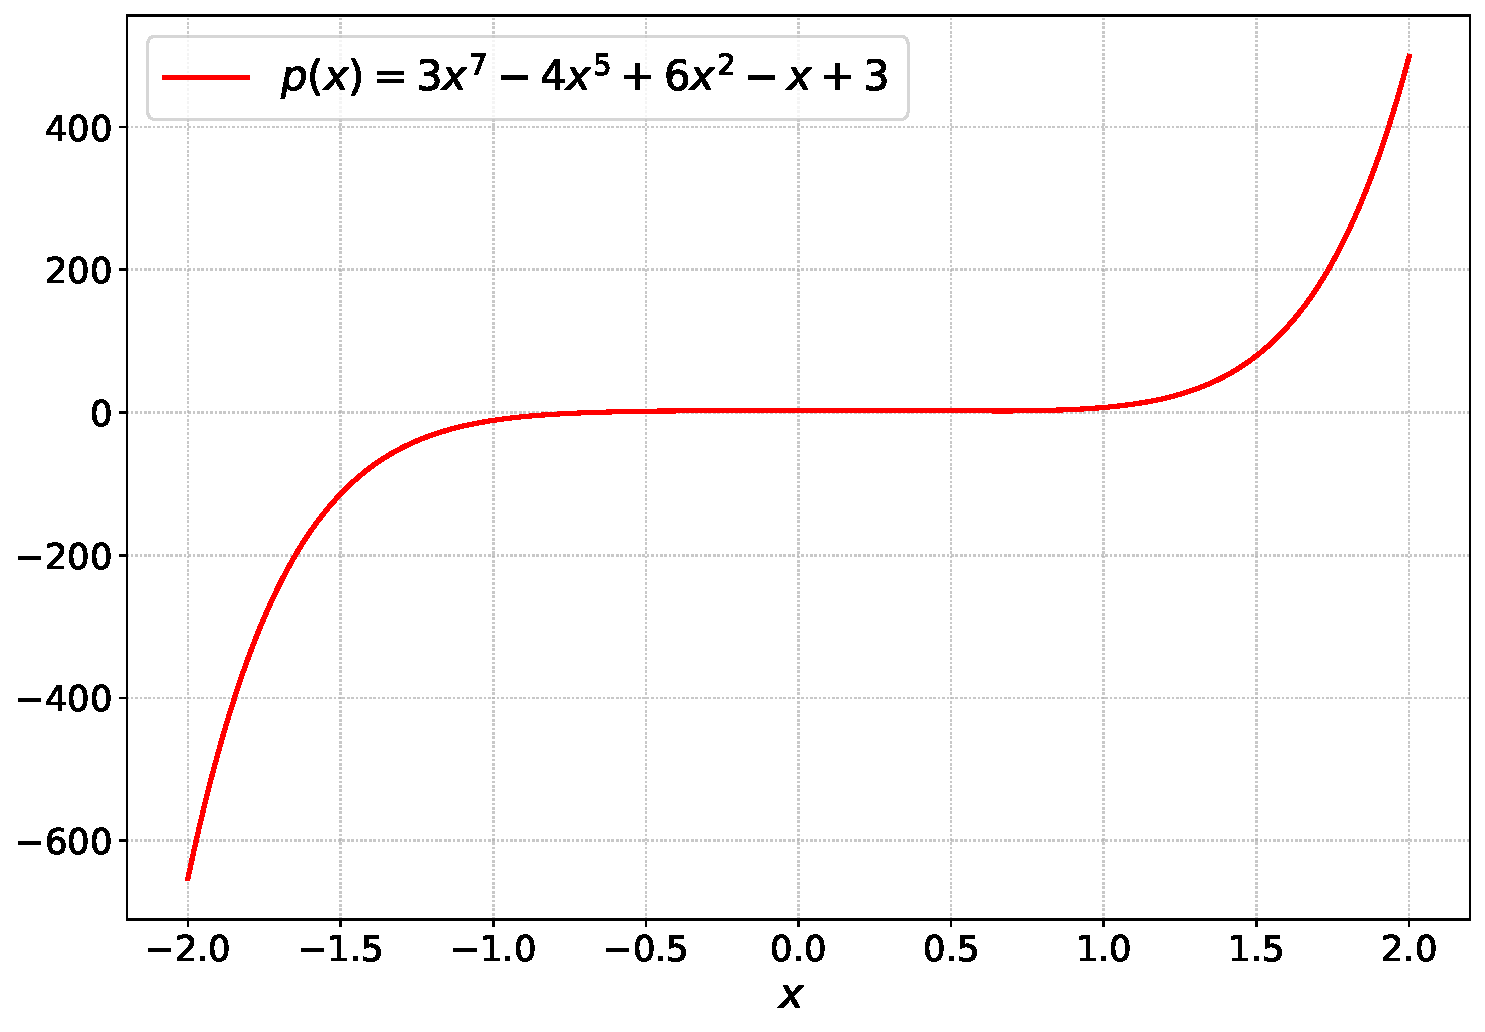
\includegraphics[width=0.8\textwidth]{polinomio.pdf}
    \caption{Gráfica de $p(x) = 3x^7 - 4x^5 + 6x^2 - x + 3$ vs $x$.}
\end{figure}
%


\begin{cajaflex}[\texttt{Resumen}]

$\blacklozenge$ Acceda a la documentación de la API (Application Programming Interface) \lstinline|numpy.polynomial| 
\href{https://numpy.org/doc/stable/reference/generated/numpy.polynomial.polynomial.Polynomial.html}{dando clic aquí}. 


\lstinline|p = np.polynomial.Polynomial(coeff)| \quad \hfill \text{\small (Creación del objeto polinomio $P(x)$)} \\
\lstinline|raices_p = p.roots()| \quad \hfill \text{\small (Cálculo de todas las raíces complejas/reales)} \\
\lstinline|valorevaluado = p(r)| \quad \hfill \text{\small (Evaluación directa en un punto o arreglo $x$)}

\textcolor{teal!60!black}{\rule{\linewidth}{0.8pt}}

\vspace{0.1cm}

\subsubsection*{\textcolor{teal!70!black}{1. \texttt{coeff = [a\_0, a\_1, ..., a\_n]}}}
La clase \texttt{Polynomial}  requiere ingresar los coeficientes en orden ascendente de 
potencias ($a_0 + a_1 x + a_2 x^2 + \dots + a_n x^n$).
Es obligatorio incluir ceros para los grados ausentes. 
Por ejemplo, en $3x^7 - 4x^5 + 6x^2 - x + 3$, las potencias $x^3, x^4, x^6$ 
se representan explícitamente con $0$.


\subsubsection*{\textcolor{teal!70!black}{2. \texttt{p = np.polynomial.Polynomial(coeff)}}}
\begin{itemize}
    \item \textbf{Qué hace:} Crea un objeto de clase algebraica que encapsula las propiedades 
    del polinomio.
    \item \textbf{Representación:} 
    Al imprimir \texttt{print(p)}, genera automáticamente la expresión 
    formateada $3.0 - 1.0\,x + 6.0\,x^2 - 4.0\,x^5 + 3.0\,x^7$.  El símbolo pude cambiarse
    \texttt{p = np.polynomial.Polynomial(coeff,symbol='t')} para que imprima
    $3.0 - 1.0\,t + 6.0\,t^2 - 4.0\,t^5 + 3.0\,t^7$
\end{itemize}

\subsubsection*{\textcolor{teal!70!black}{3. \texttt{p.roots()}}}
\begin{itemize}
    \item \textbf{Qué devuelve:} Un arreglo numérico con todas las raíces del polinomio (tanto reales como pares complejos conjugados).
    \item \textbf{Método interno:} Calcula los valores propios (autovalores) de la matriz compañera escalada para garantizar máxima estabilidad numérica.
\end{itemize}

\subsubsection*{\textcolor{teal!70!black}{4. Evaluaciones y Residuos: \texttt{p(r)}}}
\begin{itemize}
    \item \textbf{Evaluación directa:} El objeto \texttt{p} puede ser llamado como una función estándar de Python (\texttt{p(x)}), soportando escalares o arreglos de NumPy vectorizados.
    \item \textbf{Cálculo del residuo:} Evaluar el polinomio en la raíz calculada $P(r)$ permite medir el error numérico en punto flotante ($|P(r)| \approx 0$).
\end{itemize}

\end{cajaflex}

%--------------- problemas --------------------

\begin{problemas}[]
\begin{enumerate}[leftmargin=*]

\item Resuelva las siguientes ecuaciones utilizando el método gráfico y las rutinas de 
\lstinline|scipy.optimize|
\begin{enumerate}
    \item $x = 2 -e^{-x}$ 
    \item $x^3 + 2x = e^{-x}$
    \item $x = \cos x$
\end{enumerate}

\item La ley de radiación de Planck establece que la intensidad de la radiación por unidad de área y por unidad de longitud de onda $\lambda$ de un cuerpo negro a una temperatura $T$ es:
\begin{align*}
I(\lambda) = \frac{2\pi h c^2 \lambda^{-5}}{e^{hc/\lambda k_B T} - 1},
\end{align*}
donde $h$ es la constante de Planck, $c$ es la velocidad de la luz y $k_B$ es la constante de Boltzmann.

\begin{enumerate}
    \item[a)] Muestre, mediante derivación, que la longitud de onda $\lambda$ en la cual la radiación emitida es máxima es la solución de la ecuación:
    \begin{align*}
    5e^{-hc/\lambda k_B T} + \frac{hc}{\lambda k_B T} - 5 = 0.
    \end{align*}
    Realice la sustitución $x = hc/\lambda k_B T$ y demuestre a partir de ello que la longitud de onda de radiación máxima obedece la \textit{ley del desplazamiento de Wien}:
    \begin{align*}
    \lambda = \frac{b}{T},
    \end{align*}
    donde la llamada \textit{constante de desplazamiento de Wien} es $b = hc/k_B x$, y $x$ es la solución a la ecuación no lineal:
    \begin{align*}
    5e^{-x} + x - 5 = 0.
    \end{align*}

    \item[b)] Escriba un programa para resolver esta ecuación con una precisión de $\epsilon = 10^{-6}$ utilizando el método de búsqueda binaria (bisección), y encuentre así un valor para la constante de desplazamiento.

    \item[c)] La ley de desplazamiento es la base del método de \textit{pirometría óptical}, un método para medir la temperatura de objetos mediante la observación del color de la radiación térmica que emiten. El método se utiliza comúnmente para estimar las temperaturas superficiales de cuerpos astronómicos, como el Sol. El pico de la longitud de onda en la radiación emitida por el Sol se encuentra en $\lambda = 502\text{ nm}$. A partir de las ecuaciones anteriores y su valor de la constante de desplazamiento, estime la temperatura superficial del Sol.
\end{enumerate}

\item Un problema de ingeniería importante que surge en múltiples aplicaciones es la vibración de una viga empotrada en un extremo y libre en el otro. Este problema se puede analizar analíticamente, pero los cálculos se reducen a resolver la siguiente ecuación algebraica no lineal:
\begin{align*}
\cosh \beta \cos \beta = -1,
\end{align*}
donde $\beta$ se relaciona con parámetros clave de la viga a través de
\begin{align*}
\beta^4 = \omega^2 \frac{\rho A}{E I},
\end{align*}
siendo $\rho$ la densidad de la viga, $A$ el área de la sección transversal, $E$ el módulo de Young e $I$ el momento de inercia de la sección transversal. El parámetro de mayor interés es $\omega$, que representa la frecuencia angular de la viga.

Deseamos calcular las frecuencias de una viga de acero en vibración con una sección transversal rectangular de ancho $b = 25\text{ mm}$ y alto $h = 8\text{ mm}$. La densidad del acero es $\rho = 7850\text{ kg/m}^3$ y su módulo de Young es $E = 2 \times 10^{11}\text{ Pa}$. El momento de inercia de una sección transversal rectangular está dado por $I = bh^3 / 12$.

\begin{enumerate}
    \item[a)] Grafique la ecuación a resolver para que se pueda inspeccionar dónde ocurren los cruces por cero.
    
    \textit{Sugerencia:} Al escribir la ecuación como $f(\beta) = 0$, la función $f$ aumenta su amplitud de forma dramática a medida que crece $\beta$. Por lo tanto, es prudente analizar una ecuación con amplitud amortiguada, $g(\beta) = e^{-\beta} f(\beta) = 0$. Grafique la función $g$ en su lugar.

    \item[b)] Calcule las tres primeras frecuencias de la viga.
\end{enumerate}

\item Considere el polinomio de grado seis
%
\begin{align*}
   P(x) = 924x^6 - 2772x^5 + 3150x^4 - 1680x^3 + 420x^2 - 42x + 1.
\end{align*}
%
\begin{enumerate}[label=\alph*)]
   \item Realice una gráfica de $P(x)$ en el intervalo $x \in [0, 1]$. 
   A partir de la inspección visual de la gráfica, 
   estimar los valores aproximados de las seis raíces del polinomio 
   (los puntos donde la función se anula).
   
   \item Utilizando las funciones integradas de álgebra lineal de NumPy 
   (\lstinline|np.roots| o \lstinline|np.polynomial.Polynomial.roots|) 
   escriba un programa en Python para encontrar las posiciones de 
   las seis raíces y muestre sus residuos.
\end{enumerate}

\item \textbf{El punto de Lagrange:}
Existe un punto especial entre la Tierra y la Luna, conocido 
como el punto de Lagrange $L_1$, en el cual un satélite orbita alrededor 
de la Tierra en perfecta sincronía con la Luna, manteniéndose 
siempre entre ambos cuerpos. Esto ocurre porque la atracción gravitacional 
de la Tierra hacia adentro y la de la Luna hacia afuera se combinan para 
generar exactamente la fuerza centrípeta requerida para mantener al satélite
en su órbita.

\begin{enumerate}[label=\alph*)]
   \item Suponiendo órbitas circulares y que la masa de la Tierra 
   es mucho mayor que la de la Luna o el satélite, demuestre que la distancia 
   $r$ desde el centro de la Tierra al punto $L_1$ satisface la ecuación de 
   equilibrio de fuerzas:
   %
   \begin{align*}
      \frac{GM}{r^2} - \frac{Gm}{(R - r)^2} = \omega^2 r,
   \end{align*}
   %
   donde $R$ es la distancia Tierra-Luna, $M$ y $m$ son las masas de la Tierra y
   la Luna respectivamente, $G$ es la constante de gravitación universal, 
   y $\omega$ es la velocidad angular de la Luna y del satélite.

   \item Al multiplicar por $r^2(R-r)^2$ y reordenar términos, 
   demuestre que la ecuación anterior se reduce a un polinomio de grado 
   cinco en $r$:
   %
   \begin{align*}
      \omega^2 r^5 - 2\omega^2 R r^4 + \omega^2 R^2 r^3 + G(m - M) r^2 + 2 G M R r - G M R^2 = 0.
   \end{align*}

   \item Escriba un programa en Python que resuelva la posición del punto $L_1$ 
   utilizando la API de polinomios de NumPy 
   (\lstinline|np.polynomial.Polynomial.roots|). 
   Seleccione la raíz físicamente válida ($0 < r < R$) e 
   identifique las demás raíces complejas/no físicas.
   Los valores para los parámetros físicos son:
   %
   \begin{align*}
      G &= 6.674 \times 10^{-11} \text{ m}^3 \text{kg}^{-1} \text{s}^{-2}, \quad &M = 5.974 \times 10^{24} \text{ kg}, \\
      m &= 7.348 \times 10^{22} \text{ kg}, \quad &R = 3.844 \times 10^8 \text{ m}, \\
      \omega &= 2.662 \times 10^{-6} \text{ s}^{-1}.
   \end{align*}

   {\centering
\begin{tikzpicture}[>=stealth, scale=0.85]
    % Esferas / Cuerpos celestes
    \draw[fill=blue!15, double=black, thick] (0,0) circle (0.6) node {$M$};
    \node[below=0.7cm] at (0,0) {Tierra};

    \draw[fill=gray!20, thick] (8,0) circle (0.35) node {$m$};
    \node[below=0.45cm] at (8,0) {Luna};

    \filldraw[black] (5.2,0) circle (0.08);
    \node[below=0.2cm] at (5.2,0) {\small Satélite ($L_1$)};

    % Flechas de distancia
    \draw[<->, thick] (0,1.5) -- (8,1.5) node[midway, fill=violet!6!white] {$R$};
    \draw[<->, thick] (0,0.9) -- (5.2,0.9) node[midway, fill=violet!6!white] {$r$};

    % Líneas de referencia discontinuas
    \draw[gray, dotted, thick] (0,0) -- (0,1.7);
    \draw[gray, dotted, thick] (5.2,0) -- (5.2,1.1);
    \draw[gray, dotted, thick] (8,0) -- (8,1.7);
\end{tikzpicture}
\par}

\vspace{0.2cm}
\captionof{figure}{Esquema del sistema Tierra--Luna y la posición del punto $L_1$.}
\vspace{0.2cm}
\end{enumerate}

\end{enumerate}

\end{problemas}




\end{document}

